\section{Les SiPM, un détecteur de lumière}
Au plus simple, un SiPM est un composant electronique qui permet de detecter de la lumiere.

Un SiPM est une puce de silicium qui contrairment au processueur qui sont composer de transistors, est composer d'une multitude de photodiodes. Une photodiodes est un composant electronique qui permet de convertir de la lumiere en courant electrique. C'est notament ce qui est utiliser dans les cellules photovoltaique des panneaux solaire. Ici les photodiodes vont plutot etre optimiser pour detecter des photon que pour generer de l'electriciter. 

En temps normal, une jonction p-n est un assemblage de deux matériaux semi-conducteurs qui aggisse comme une diode (voir \cref{fig_pn_diode}). Un choisissant judicisement ses materieux et en lui appliquant une tension dans son sense conventionele on peut obtenir l'emition de lumiere. C'est le principe de la LED. En revanche, si on applique une tension dans le sens inverse alors le courant ne peut plus circuler car c'est une diode. Quand un photon d'une energie suifisant vient frapper la jonction, il va liberer un electron qui va creer un courant electrique proportionel au nombre de photon qui . C'est le principe de la photodiode.

Notre detecteur peut etre plus sensible si nous augmenton la tention alors nous commencon a observer un phenomene d'avalanche. En effet, quand une paire electron-trou est crée, elle va accelerer dans le champ electrique et liberer d'autre paire electron-trou. C'est le principe du photodetecteur avalache (APD)
(avalanche photodetector) mais nous arrivons rapidement a une limite; A une certaine tention, dite la tenstion de claquage, la diode va se mettre a conduire dans le sens inverse. Dans ce cas le photon que nous detecterons en premier créra un courant qui s'entrenindras tous suel. Pour empecher cela il fout donc limiter le courant du signal. Dans le cas des SiPM, cela est fait avec une reistance et une accumulateur pour former ce qu'on appelera un SPAD (Single photon avalanche diode).

Dans un SiPM, nous allons relier en parrale des centain voir des millier de ces SPAD (voir \cref{fig_SiPM}). Ainsi, on augment la surface de detection pour un photon. Acctuelement, dans le commerce la taille la plus grande de SiPM disponile est de 8mm*8mm \cite{}. En couplant plusieur SiPM en parralelle, on peut donc detecter des photons sur une surface plus grande.

\begin{figure}
    \centering
    % \begin{subfigure}{0.45\textwidth}
    %     \centering
    %     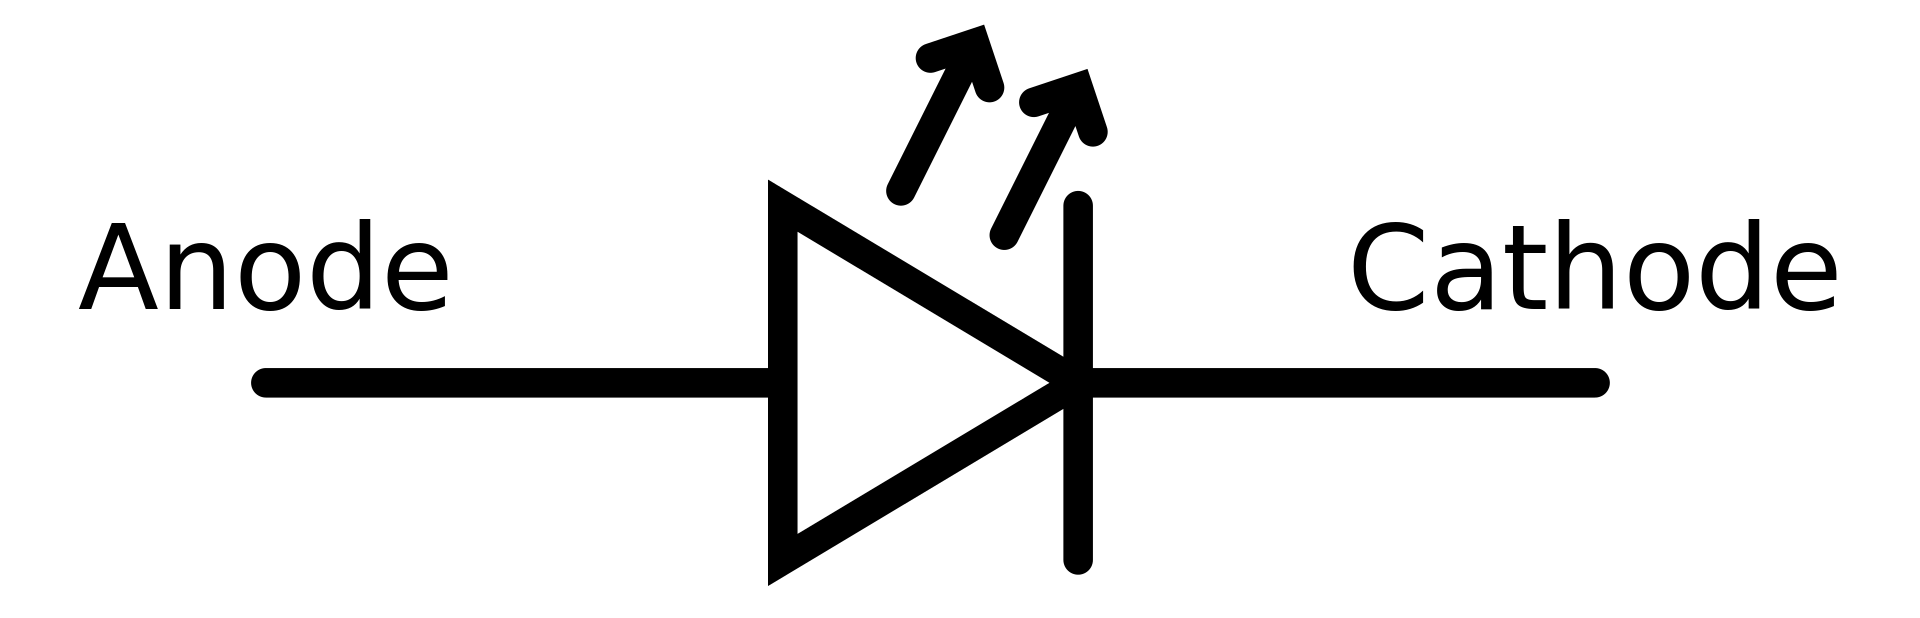
\includegraphics[width=\textwidth]{img/she/LED_symbol.svg.png}
    %     \captionsetup{width=.85\textwidth}
    %     \caption{Source: \href{https://commons.wikimedia.org/wiki/File:LED_symbol.svg}{Omegatron}, \href{https://creativecommons.org/licenses/by-sa/3.0}{CC BY-SA 3.0}, via Wikimedia Commons}
    %     \label{fig_LED_elec_symbol}
    % \end{subfigure}
    % \begin{subfigure}{0.45\textwidth}
    %     \centering
    %     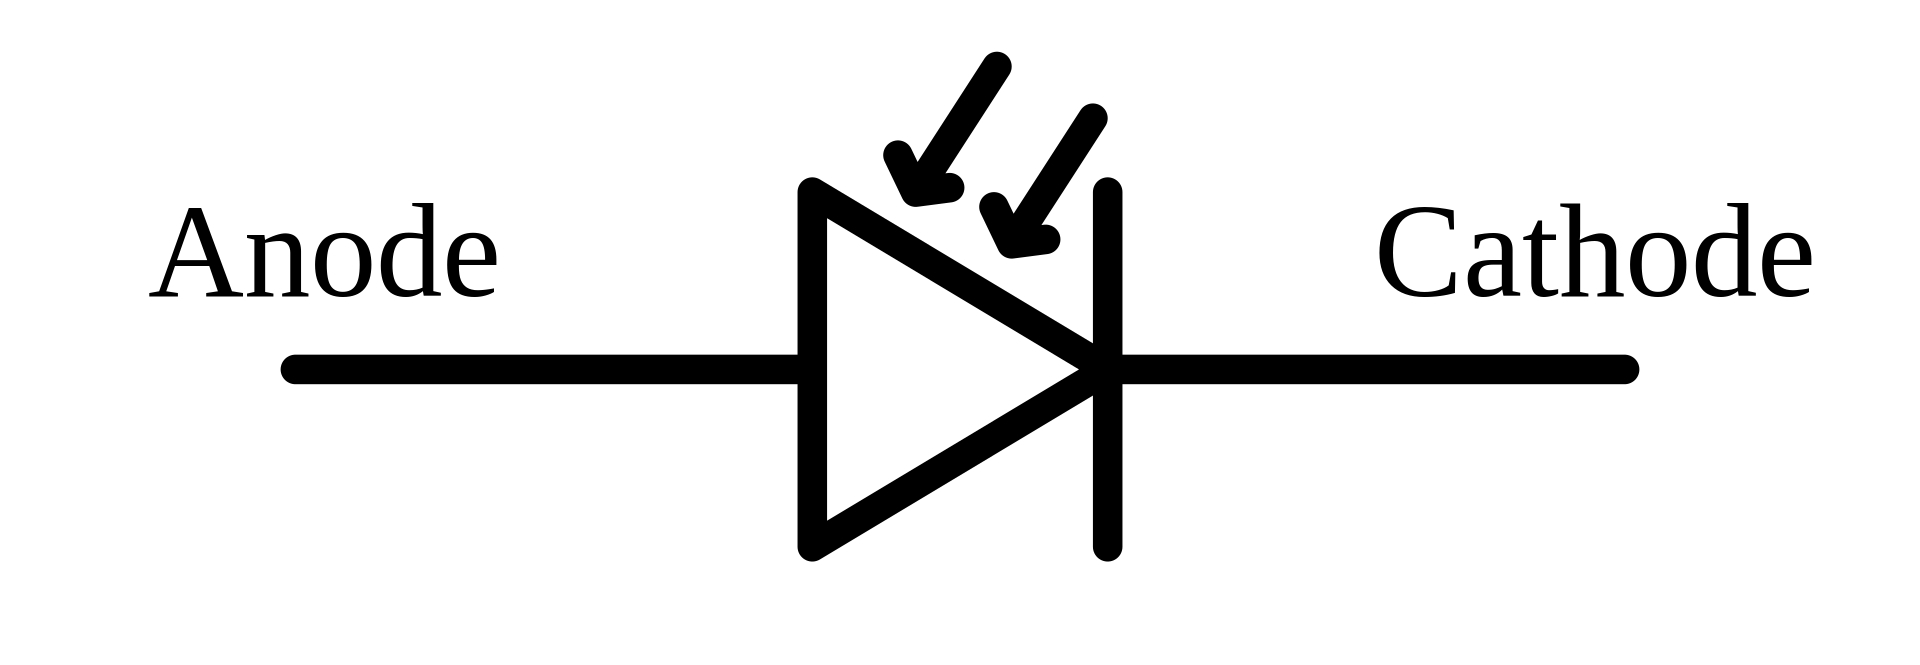
\includegraphics[width=0.85\textwidth]{img/she/Photodiode_symbol.svg.png}
    %     \captionsetup{width=.85\textwidth}
    %     \caption{Source: \href{https://commons.wikimedia.org/wiki/File:Photodiode_symbol.svg}{Simone Biancolilla}, \href{https://creativecommons.org/licenses/by-sa/3.0}{CC BY-SA 3.0}, via Wikimedia Commons}
    %     \label{fig_photodiode_elec_symbol}
    % \end{subfigure}
    \begin{subfigure}{0.45\textwidth}
        \centering
        \raisebox{0.25\textwidth}{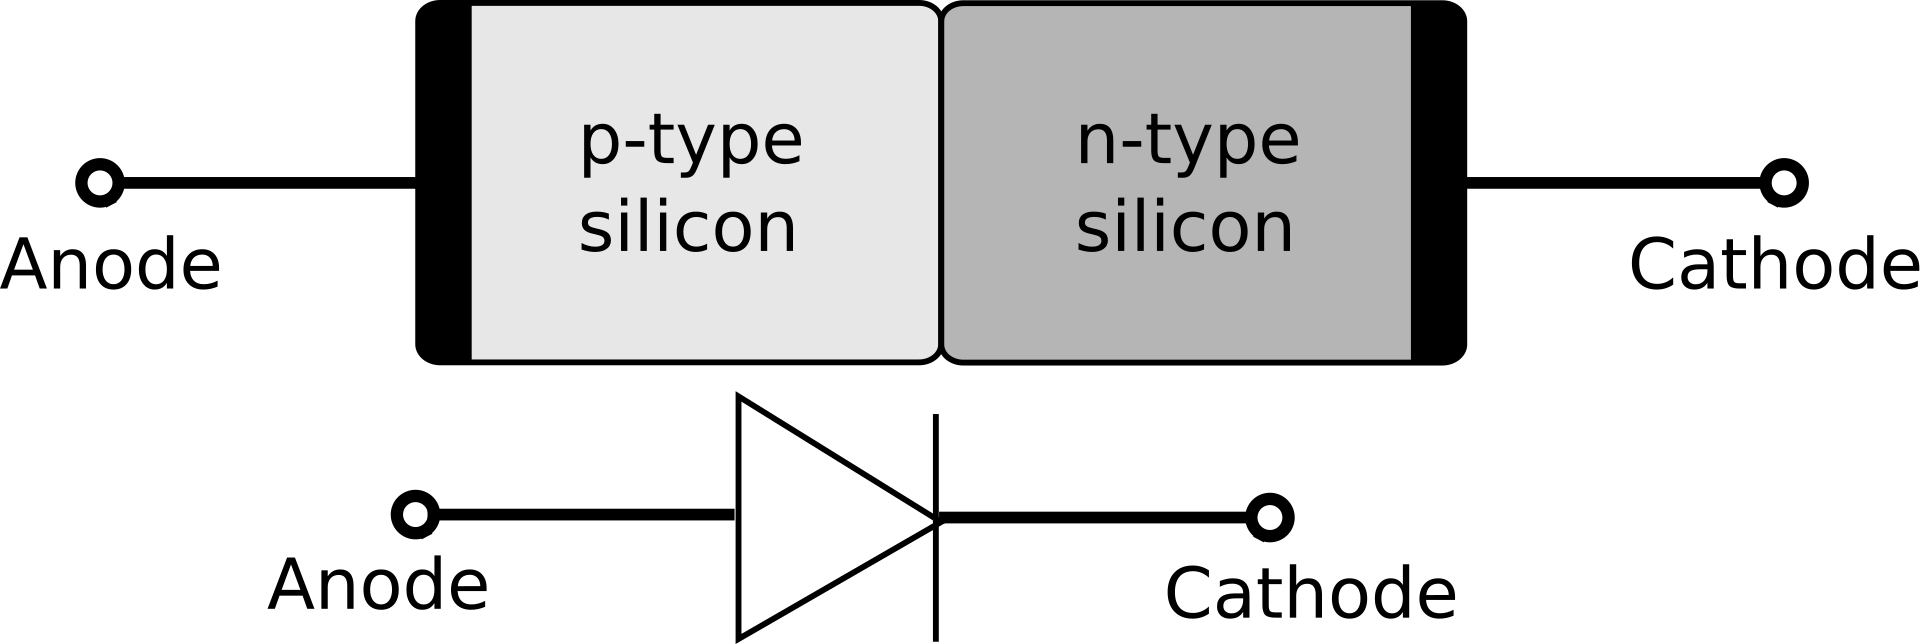
\includegraphics[width=0.85\textwidth]{img/she/1920px-PN_diode_with_electrical_symbol.svg.png}}
        \captionsetup{width=.85\textwidth}
        \caption{Shema montrant l'equivalence entre une jonction P-N et une diode. Source: \href{https://commons.wikimedia.org/wiki/File:PN_diode_with_electrical_symbol.svg}{Raffamaiden}, \href{https://creativecommons.org/licenses/by-sa/3.0}{CC BY-SA 3.0}, via Wikimedia Commons}
        \label{fig_pn_diode}
    \end{subfigure}
    \begin{subfigure}{0.45\textwidth}
        \centering
        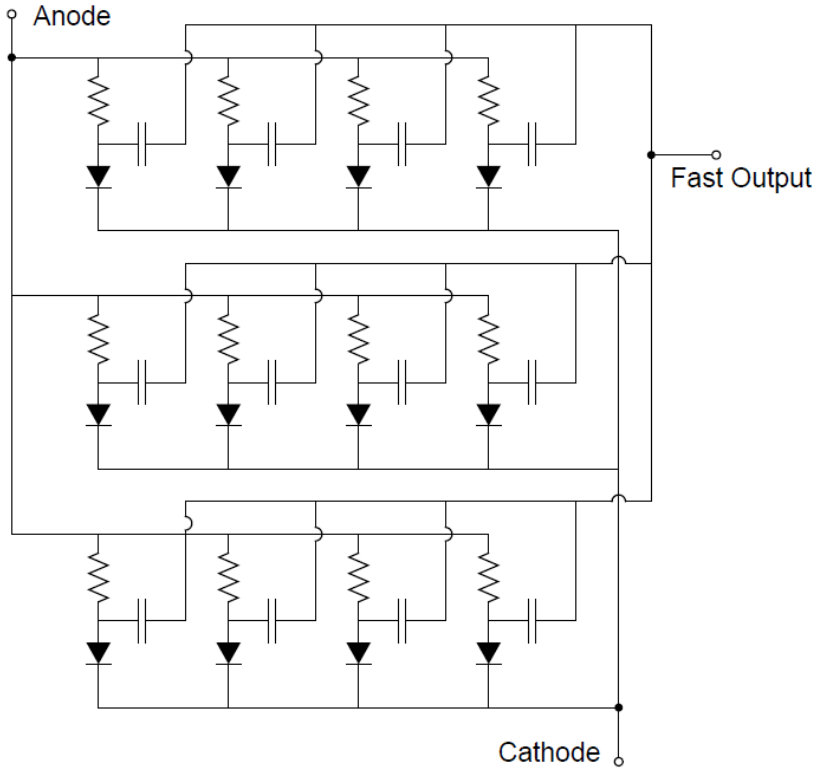
\includegraphics[width=0.85\textwidth]{img/she/SiPM_arithecture.png}
        \captionsetup{width=.85\textwidth}
        \caption{Schéma d'un SiPM. Les diode sont des diode photoavalanche. On ne reprensent pas touts les module. Source~:~\href{https://websites.umich.edu/~ners580/ners-bioe_481/lectures/pdfs/2017-02-.pdf}{An Intro to SiPM, SensL}}
        \label{fig_SiPM}
    \end{subfigure}
    \caption[Composition d'un SiPM]{Composition d'un SiPM}
\end{figure}
